
\section{Главный фактор загрязнения воздуха}
\begin{frame}{\insertsectionhead}
    \begin{minipage}{0.55\textwidth}
        \footnotesize
        Основным фактором загрязнения атмосферы
        являются автомобили, количество которых
        с каждым годом увеличивается.

        \medskip

        В процессе эксплуатации автомобиля выделяется большое количество
        вредных веществ, таких как монооксид углерода, оксиды азота, 
        углеводороды, альдегиды, сажа, бензпирен-3.4.

    \end{minipage}
    \begin{minipage}{0.43\textwidth}
        \tiny
        Количество атмомобилей в собственности граждан
        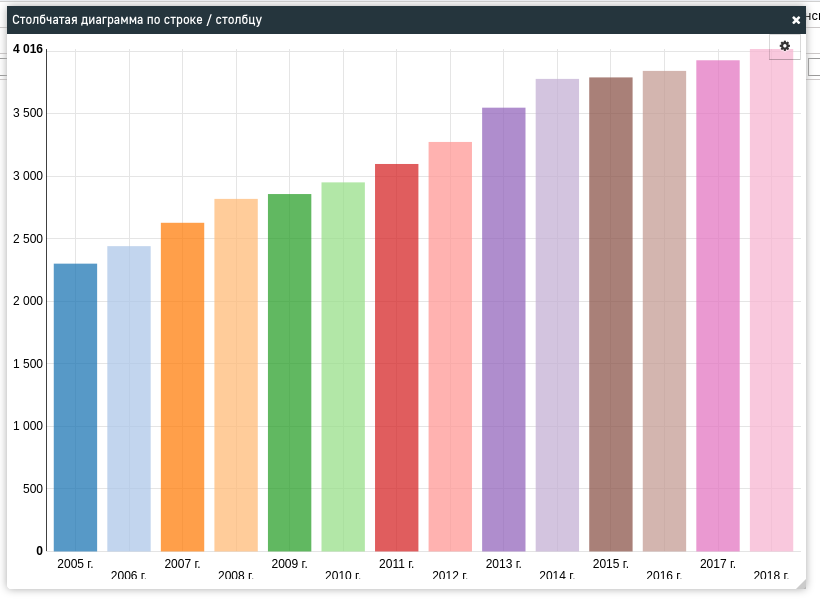
\includegraphics[width=\textwidth]{assets/car_stats.png}
    \end{minipage}
\end{frame}

